% begin module related-rates-ex1

\begin{frame}
\begin{example}
A plane flies directly overhead of you  \alertNoH{ 8}{ at $500$ km/h} maintaining an altitude of
$3$ km.  \alertNoH{ 10}{ How fast is the plane's distance from you increasing} at the
moment  \alertNoH{ 10}{when the plane is flying over a point on the ground $4$ km
from you}? \pause 
\begin{itemize}
\item We'll use our general guideline to solve this problem. To start, \textbf{draw a picture} and introduce variables/labels. \end{itemize} \pause 
\begin{columns}[c]
\column{.33\textwidth}

%To include the image below, be sure to include the following in preamble
%\usepackage{bbding}
%\let\Cross\relax
%\let\Square\relax

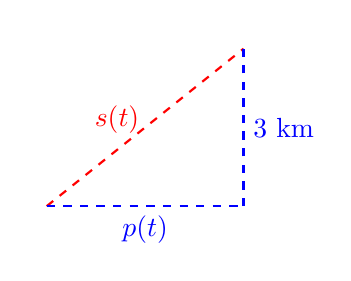
\begin{tikzpicture}[scale=.5]
\draw[color=red, dashed,  thick] (0,0) -- (5,4);
%\draw[penColor, dashed, thick] (0,0) -- (0,4);
\draw[color=blue, dashed, thick] (5,0) -- (5,4);
\draw[color=blue, dashed, thick] (0,0) -- (5,0);
%\draw[|->,color=blue, dashed] (2.7,2.5) -- (4.8,4.1);
\node [left,color=green] at (5.7,4.3) {\scalebox{1.5}{\Plane}};
%note: \Plane required the bbding package
%\draw [color=blue, fill] (5,4) circle [radius=.07];
\node [left,color=blue] at (0,0) {\scalebox{3} {\Ladiesroom} 
};
\node [right,color=blue] at (5,2) {$3$ km};
%\node [above,color=blue] at (3,4) {$p'(t) = 500$ mph};
\node [below,color=blue] at (2.5,0) {$p(t)$};
\node [left,color=red] at (2.6,2.2) {$s(t)$};
\end{tikzpicture} \pause 
\column{.65\textwidth}
 \pause 
 At time $ t $ (hours), let\\
 $p=p(t)$  be the distance (km) between you and the point on the ground directly below the plane,\\ \vspace*{2mm}
$ s=s(t) $  be the distance (km) between yourself and the plane.\\
 \pause \vspace*{2mm}
 
\textbf{ Identify and given and required rates:}\\ \vspace*{2mm}
\pause 

Given: \pause  \alertNoH{ 8}{ ${\frac{\diff p}{\diff t} = p'(t)=500}$ km/h} \pause \\ \vspace*{2mm} 

Required: \pause Find  \alertNoH{ 10}{ $ \frac{\diff s}{\diff t}=s'(t) $} when  \alertNoH{ 10}{$ p=4.$} 
\end{columns}

\end{example}
\end{frame}


\begin{frame}
\begin{example}
\begin{columns}[c]
\column{.33\textwidth}
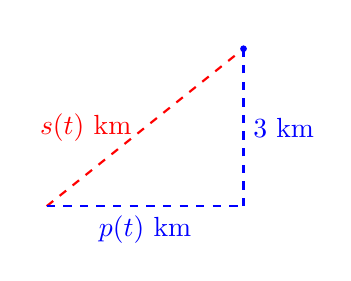
\begin{tikzpicture}[scale=.5]
\draw[color=red, dashed,  thick] (0,0) -- (5,4);
%\draw[penColor, dashed, thick] (0,0) -- (0,4);
\draw[color=blue, dashed, thick] (5,0) -- (5,4);
\draw[color=blue, dashed, thick] (0,0) -- (5,0);
%\draw[->,color=blue, thick] (4,4) -- (6,4);
\node [left,color=green] at (5.7,4.3) {\scalebox{1.5}{\Plane}};
%note: \Plane required the bbding package
\draw [color=blue, fill] (5,4) circle [radius=.07];
\node [left,color=blue] at (0,.5) {\scalebox{3} \Ladiesroom};
%\node [right,color=blue] at (6,4) {\scalebox{3}{\ding{40}}};
\node [right,color=blue] at (5,2) {$3$ km};
%\node [above,color=blue] at (3,4) {$p'(t) = 500$ mph};
%\node [above,color=blue] at (5,4) {$p(t)$};
\node [below,color=blue] at (2.5,0) {$p(t)$ km};
\node [left,color=red] at (2.4,2) {$s(t)$ km};
\end{tikzpicture}
\column{.65\textwidth}
 
 Given:      $\ds p'(t)= 500$ km/h  \\
 Required: $ \ds s'(t) $ when $ p=4.$ \pause \\
\textbf{Find an equation}  relating quantities with given/required rates:  \pause (ty Pythagoras)
\[
p^2+3^2=s^2
\]   \pause 
\end{columns}


\textbf{Differentiate} (implicitly with respect to $ t $):
\[
2p\cdot p'(t)+ 0 =2s\cdot s'(t)
\]
\pause 
Now \textbf{evaluate} when  $p(t)=4$ and $p'(t) =
500$.\\ \pause 
Additionally, we know that when $ p(t)=4 $ we have  $s^2=p^2+3^2=16+9=25$, so
$s=5$.  \pause 
Putting this all into our last equation we get
\[
2(4)(500)=2(5)s'(t),
\]
thus $s'(t)=400$ km/h.
\end{example}
\end{frame}

% end module related-rates-ex1
